\documentclass{article}

\usepackage[utf8]{inputenc}
\usepackage{geometry}
\usepackage{glossaries}
\usepackage[english]{babel} 
% \usepackage{biblatex}
\usepackage{hyperref}

% \geometry{
%  a4paper,
%  total={165mm,250mm},
%  left=25mm,
%  top=30mm,
%  }
 \usepackage{graphicx}
%  \usepackage{titling}

\title{Results of Using Task Knowledge}
\author{Christian Bauer}
% \date{ 2022}
 
 \usepackage{fancyhdr}

% * What you see
% * How much we defer from the real value
% * And why we see the difference and explain the reason (algorithm, data...)


\begin{document}

  \maketitle

  \section{Preliminary}
  
    In this section, two Long-Short-Term Memory \cite{hochreiterLongShortTermMemory1997} (LSTM) models 
    are compared with the actual utilization and the user allocated utilization.
    Since user allocated utilization is also a kind of prediction, in this case, a human made prediction, we will further on refer to it as one of the types of prediction.  The user has to predefine the required hardware allocation before submitting the task to the system.
    \begin{quote}
      A commonly known problem in resource management is that users often request more resources than their applications actually use \cite{thonglekImprovingResourceUtilization2019}.
    \end{quote}
    The difference of the LSTM models is the feature set they were trained on, while the \nameref{par:nt-model} has no knowledge about the type of task,
    the \nameref{par:wt-model} is trained with this knowledge in order to be able to make more accurate predictions.
    The layer architecture and hyper-parameters are the same for both models except for the feature set to be able to isolate the performance improvement when additionally including the task type.

    \textbf{TODO DESCRIBE SEQUENTIAL DATA IN A FEW WORDS?}
    
  
  \paragraph*{NT-Model}
  \label{par:nt-model}

    The LSTM model denoted as \emph{NT-model}, 
    where NT is short for \emph{no tasks} was trained without any knowledge of the task type.
    This LSTM model is solely trained on the information of how much CPU and memory is allocated for the tasks in a sequence and how much CPU and memory capability are available in total for each resource.
  
  \paragraph*{WT-Model}
  \label{par:wt-model}

    The LSTM model denoted as \emph{WT-model}, where \emph{WT} is short for \emph{with tasks} was trained with knowledge about the task types in a sequence of tasks additionally to the information
    that was available to the \nameref*{par:nt-model}.
    A task type in this scenario is either a machine learning training task, a parallel computational task, 
    a storage task, encoding/decoding task or a microservice task used to communicate with other microservices.
    The task types are categorical data, that first is \emph{one-hot encoded} \cite{seger2018investigation} \cite{yu2022missing} and then appended to the dataset that will be fed to the LSTM model while training.
    The task types were obtained by clustering similar tasks together into clusters and while run-time.
    Then the tasks in the pipeline are assigned to the clusters in order that the LSTM model can use the additional information for the prediction.

  \paragraph{How to Read the Figures}
  \label{par:how-to-read-figures}

    In the figures \ref{fig:cpu-prediction}, \ref{fig:mem-prediction}, the black line represents the values of the actual respective hardware utilization.
    The dotted grey line represents the hardware utilization that was allocated by a user for that task. The above stated tendency to over-allocate resources holds for the analyzed dataset. 
    The blue line represents the predicted hardware utilization that was made by the LSTM \nameref{par:nt-model}.
    This LSTM model is not able to react to hardware changes inside the system as fast and finely as the LSTM that was also provided the task type information.
    The green line represents the predicted hardware utilization that was made by the LSTM \nameref{par:wt-model}.

    For both the CPU and memory allocation analysis, the x-axis represents the order of tasks inside the sequential data that is called \emph{time step} in the figures.
    In the CPU prediction figure \ref{fig:cpu-prediction}, the y-axis visualizes the amount of used/allocated CPU cores in percentage. This means if a task is using 4 cores in total, it will be displayed as $400$ in the y-axis in the figure.
    In the memory prediction figure \ref{fig:mem-prediction}, the y-axis displays the space of used/allocated memory in gigabytes. Meaning a task that uses $8$ gigabytes of memory space will be displayed as $8$ on the y-axis in the figure.

    For better visibility, only a small portion of the actual dataset is shown in the figures (ranging from 3000 to 3500).
    The dataset used for the evaluation consists of 10 thousand sequential data points in total.

  \paragraph{How to Read the Tables}
  \label{par:how-to-read-tables}

    In the tables \ref{tab:numerical-values-of-cpu-prediction-variants}, the three predictions are compared with each other using the statistic measures \emph{mean, standard deviation} and \emph{percentile}.  
    This is calculated for each dataset of predictions and later concatenated to compare the performance of all three prediction variants.
    Before computing these measures, all values of each prediction were divided by the respective actual value of each task row in order to have a relative comparison to the actual value. Therefore, the closer the value is to $1$, the better is the result.
    Resulting values $\geq 1$ are considered as over-allocated and values $\le 1$ as under-allocated. 
    Over-, or under-allocated datasets are analyzed separately for every prediction variant.
    This separation is done to omit seemingly good results shown in the tables in case a prediction variant heavily under-allocates hardware resources.
    
    Note that this calculation has a caveat that having either the denominator or nominator but not both close to zero, the resulting value is immensely high. For that reason values are only taken into account up to the $95\%$ percentile, and neglected afterwards.

    The \emph{amount} value represents the percentage of values in the predicted dataset that were either over-, or under-allocated. Combined they do add up to $100\%$ for the whole dataset of a prediction.
    The amount of over-, under-allocation in itself is no measure about the overall performance of a prediction, only about the tendency a prediction might take. In combination with the following metrics the amount does provide valuable information about the prediction performance.
    This value is used to analyze if a prediction variants tends to over-, or under-allocate hardware resources.
    The \emph{mean} value represents the average value (or expected value) over all values of a prediction dataset. The closer this value is to $1$, the better the overall prediction. This holds for tables of both categories.
    The \emph{std} value represents the standard deviation that is calculated for each prediction dataset separately.
    It is a measure of the amount of variation of the values in the dataset. Also a low standard deviation is an indicator that values are likely to be closer to the \emph{mean}. Therefore, a lower standard deviation value is preferable to a high value.
    The \emph{min/max} values represent the minimum/maximum values in each dataset.
    The \emph{percentiles} $25\%, 50\%, 75\%$ represent the $k$-th percentiles. The percentile is a score that is below a certain percentage $k$. For example, $k = 50\%$ includes all values that are below the \emph{median}.
    The numerical results such as mean, standard deviation, etc. are always calculated from the entire dataset.

  \paragraph{How to Read the Histograms}
  \label{par:how-to-read-histograms}

    TODO
  
\pagebreak
  \section{Results}

    In the figures \ref{fig:cpu-prediction} and \ref{fig:mem-prediction}, the black line represents the values of the actual utilization.
    The dotted grey line represents the hardware utilization that was allocated by a user for that task.
    The blue line represents the predicted hardware utilization that was made by the LSTM \nameref{par:nt-model}.
    The green line represents the predicted hardware utilization that was made by the LSTM \nameref{par:wt-model}.

  \subsection{CPU Results}
  \label{sec:cpu-results}

    % In this section, a comparison will be made if the prediction of the utilization can be improved, 
    % if the ML model additionally to the CPU/MEM allocation also gets information about which type of task it is. 
    % Task types could be things like a machine learning task, an encoding task and so on.

    In this section, the different types of predictions are compared.
    
    \begin{figure}[h!]
      \centering
      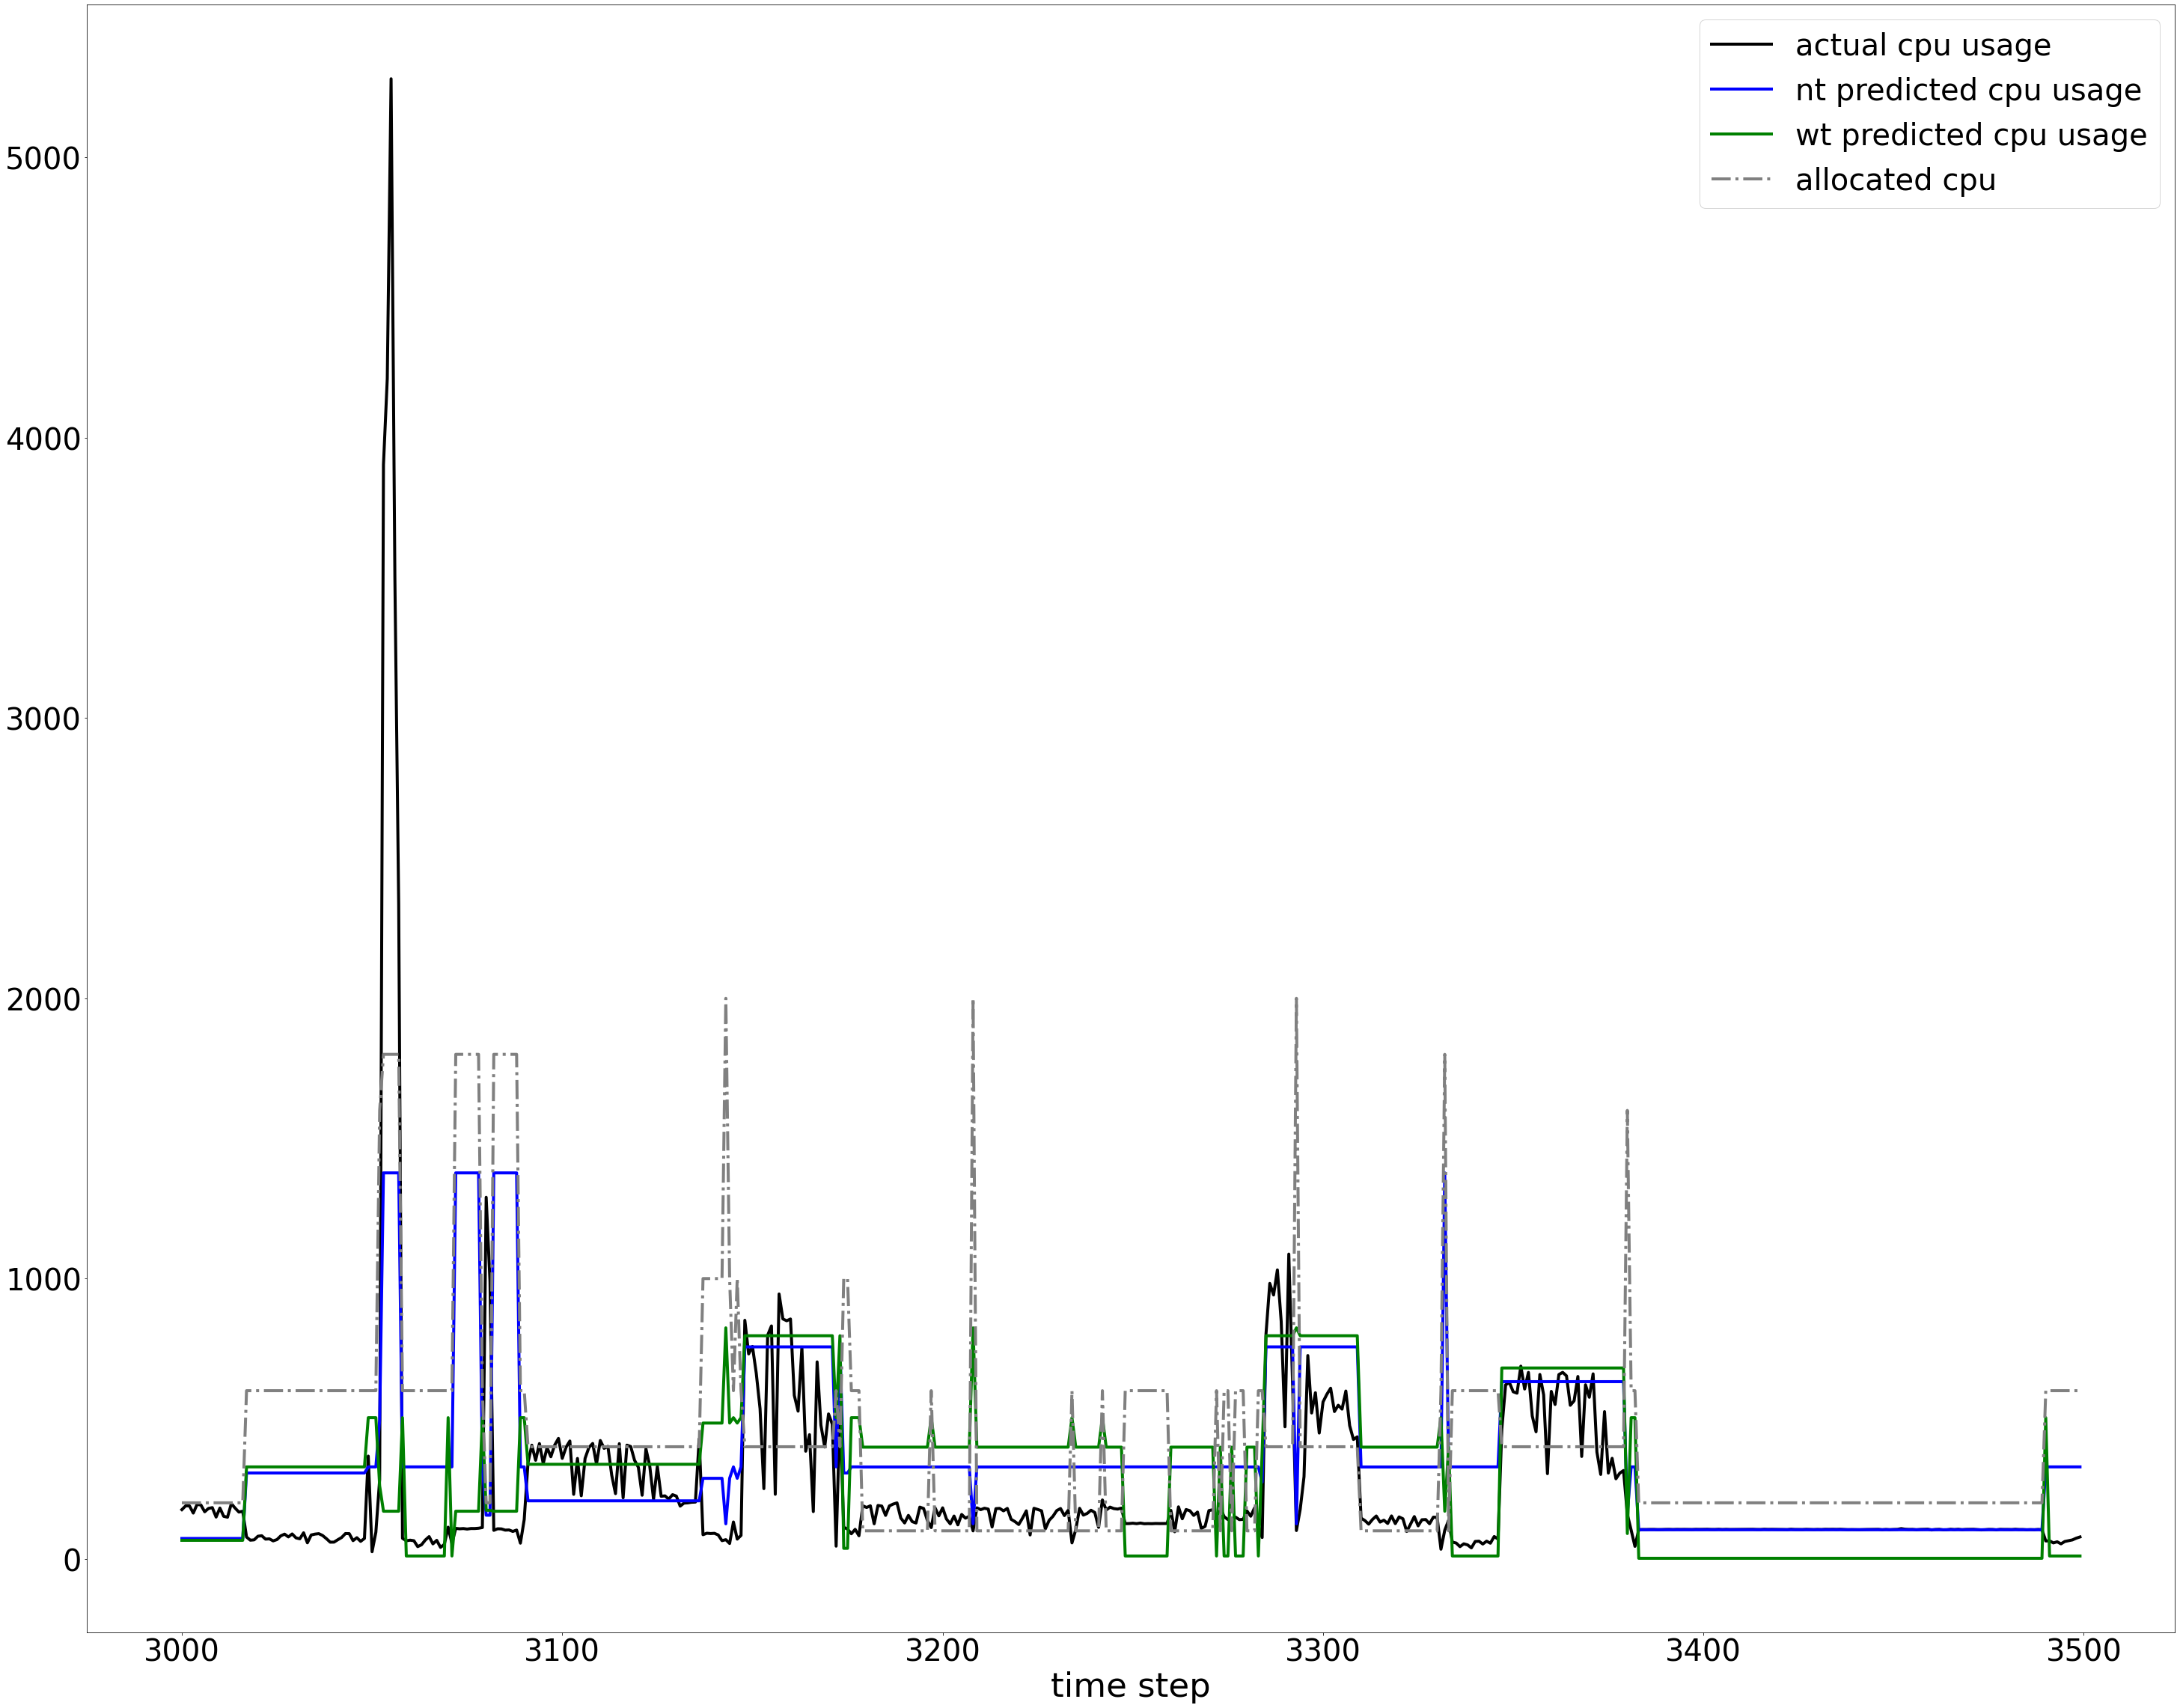
\includegraphics[width=0.85\textwidth]{figures/training_cpu_prediction.png}
      \caption{CPU Prediction}
      \label{fig:cpu-prediction}
    \end{figure}
    As can be seen in the figure, the LSTM \nameref{par:wt-model} was able to predict the actual CPU utilization the best of all three prediction modes overall.
    This is most evident when CPU utilization drops or spikes happen, were the LSTM model trained with knowledge about the task type performed best.
    None of the prediction variants was able to properly predict the large CPU utilization spike that occurs at time step $3060$. For this task, the user-based prediction had the best performance. Yet, even the user predicted allocation was off by approximately 3000. This large CPU spike is happening because this task requires numerous instances, which are not accounted for in the LSTM model versions.

    In table \ref{tab:numerical-values-of-cpu-prediction-variants}, only over-allocated predictions are taken into account.
    As can be seen, the allocation prediction done by the user over-allocates the most of all three prediction variants.
    The LSTM \nameref{par:wt-model} tends under-allocate resources rather than over-allocate. This variant also has the lowest \emph{mean} and \emph{standard deviation} values, meaning it was closest to the actual CPU utilization of all three variants for most of the values.
    All three predictions are close to the value $1$ for the \emph{minimum}, therefore all could at least once actually predict the actual CPU utilization.
    In terms of percentiles, the \nameref{par:wt-model} outperformed both the user predicted allocation and the \nameref{par:nt-model} up to the $50\%$ percentile, and afterwards was outperformed by the \nameref{par:nt-model} at the $75\%$.
    In all shown metrics the user predicted allocation performed the worst.
    

    \begin{table}
      \centering
      \begin{tabular}{|l|rrr|}
        \hline
        {} &  \textbf{Allocated CPU} &  \textbf{NT CPU Prediction} &  \textbf{WT CPU Prediction} \\
        \hline
        amount (\%) &        69.28&             61.96 &             46.47 \\
        mean  &       4.716589 &                3.117077 &                2.940870 \\
        std   &       3.679460 &                2.241624 &                2.103723 \\
        min   &       1.000012 &                1.000232 &                1.000207 \\
        25\%   &       1.903068 &                1.549565 &                1.402918 \\
        50\%   &       3.510183 &                2.374176 &                2.029432 \\
        75\%   &       6.204604 &                3.824869 &                4.102404 \\
        max   &      18.255046 &               12.907610 &               10.755826 \\
        \hline
        \end{tabular}
        \caption{Numerical Values of Over-Allocated Predictions}
        \label{tab:numerical-values-of-cpu-prediction-variants}
    \end{table}
  
      \begin{figure}[h!]
        \centering
        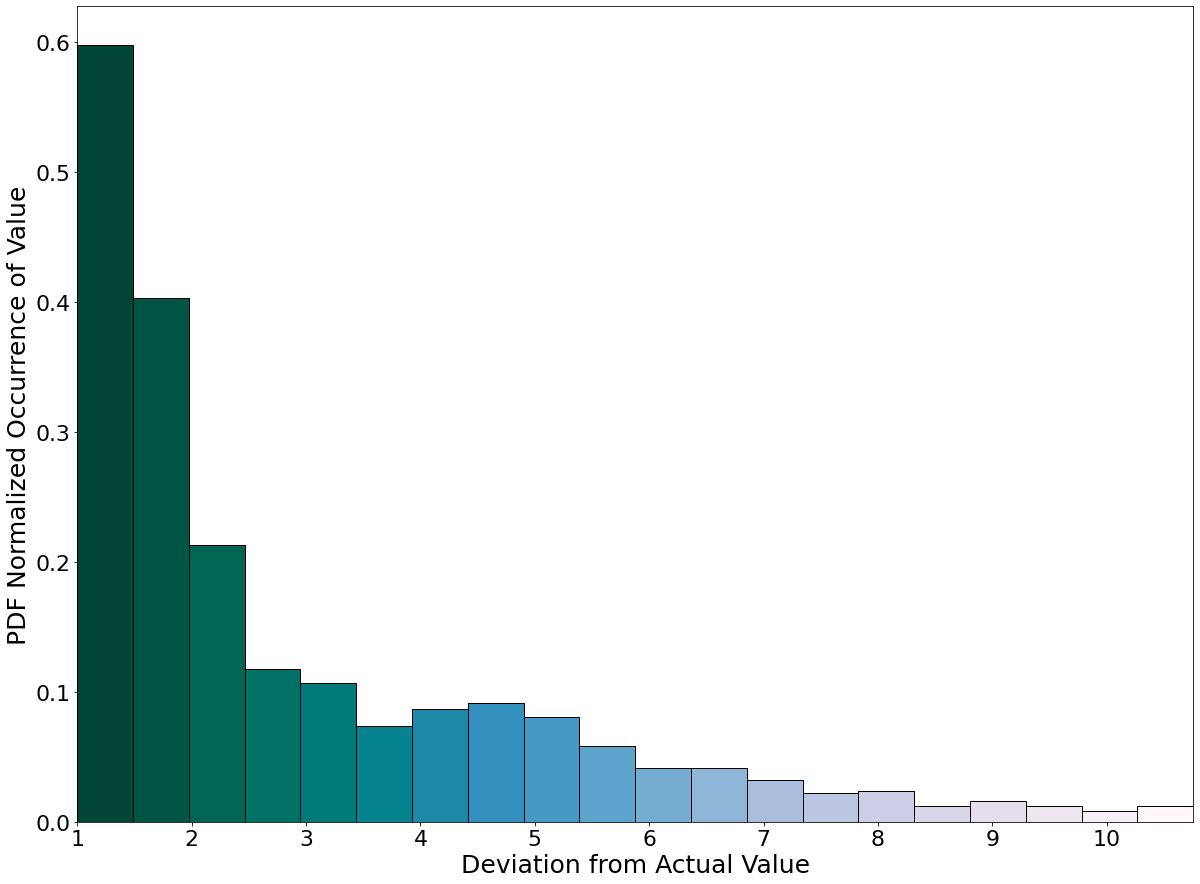
\includegraphics[width=0.85\textwidth]{figures/wt_over_aloc_hist.png}
        \caption{\nameref{par:wt-model} Prediction Histogram}
        \label{fig:wt-over-aloc-hist}
      \end{figure}

  \subsection{Memory Results}
  \label{sec:mem-results}

    Similar to the CPU utilization results, the LSTM \nameref{par:nt-model} had the best prediction performance of all three variants. In terms of memory wastage, the predicted memory allocation created by the user had the worst overall performance as can be seen in figure \ref{fig:mem-prediction}.
    % TODO HERE MAYBE ADD PERCENTAGE OF WASTAGE
    

    \begin{figure}[!ht]
      \centering
      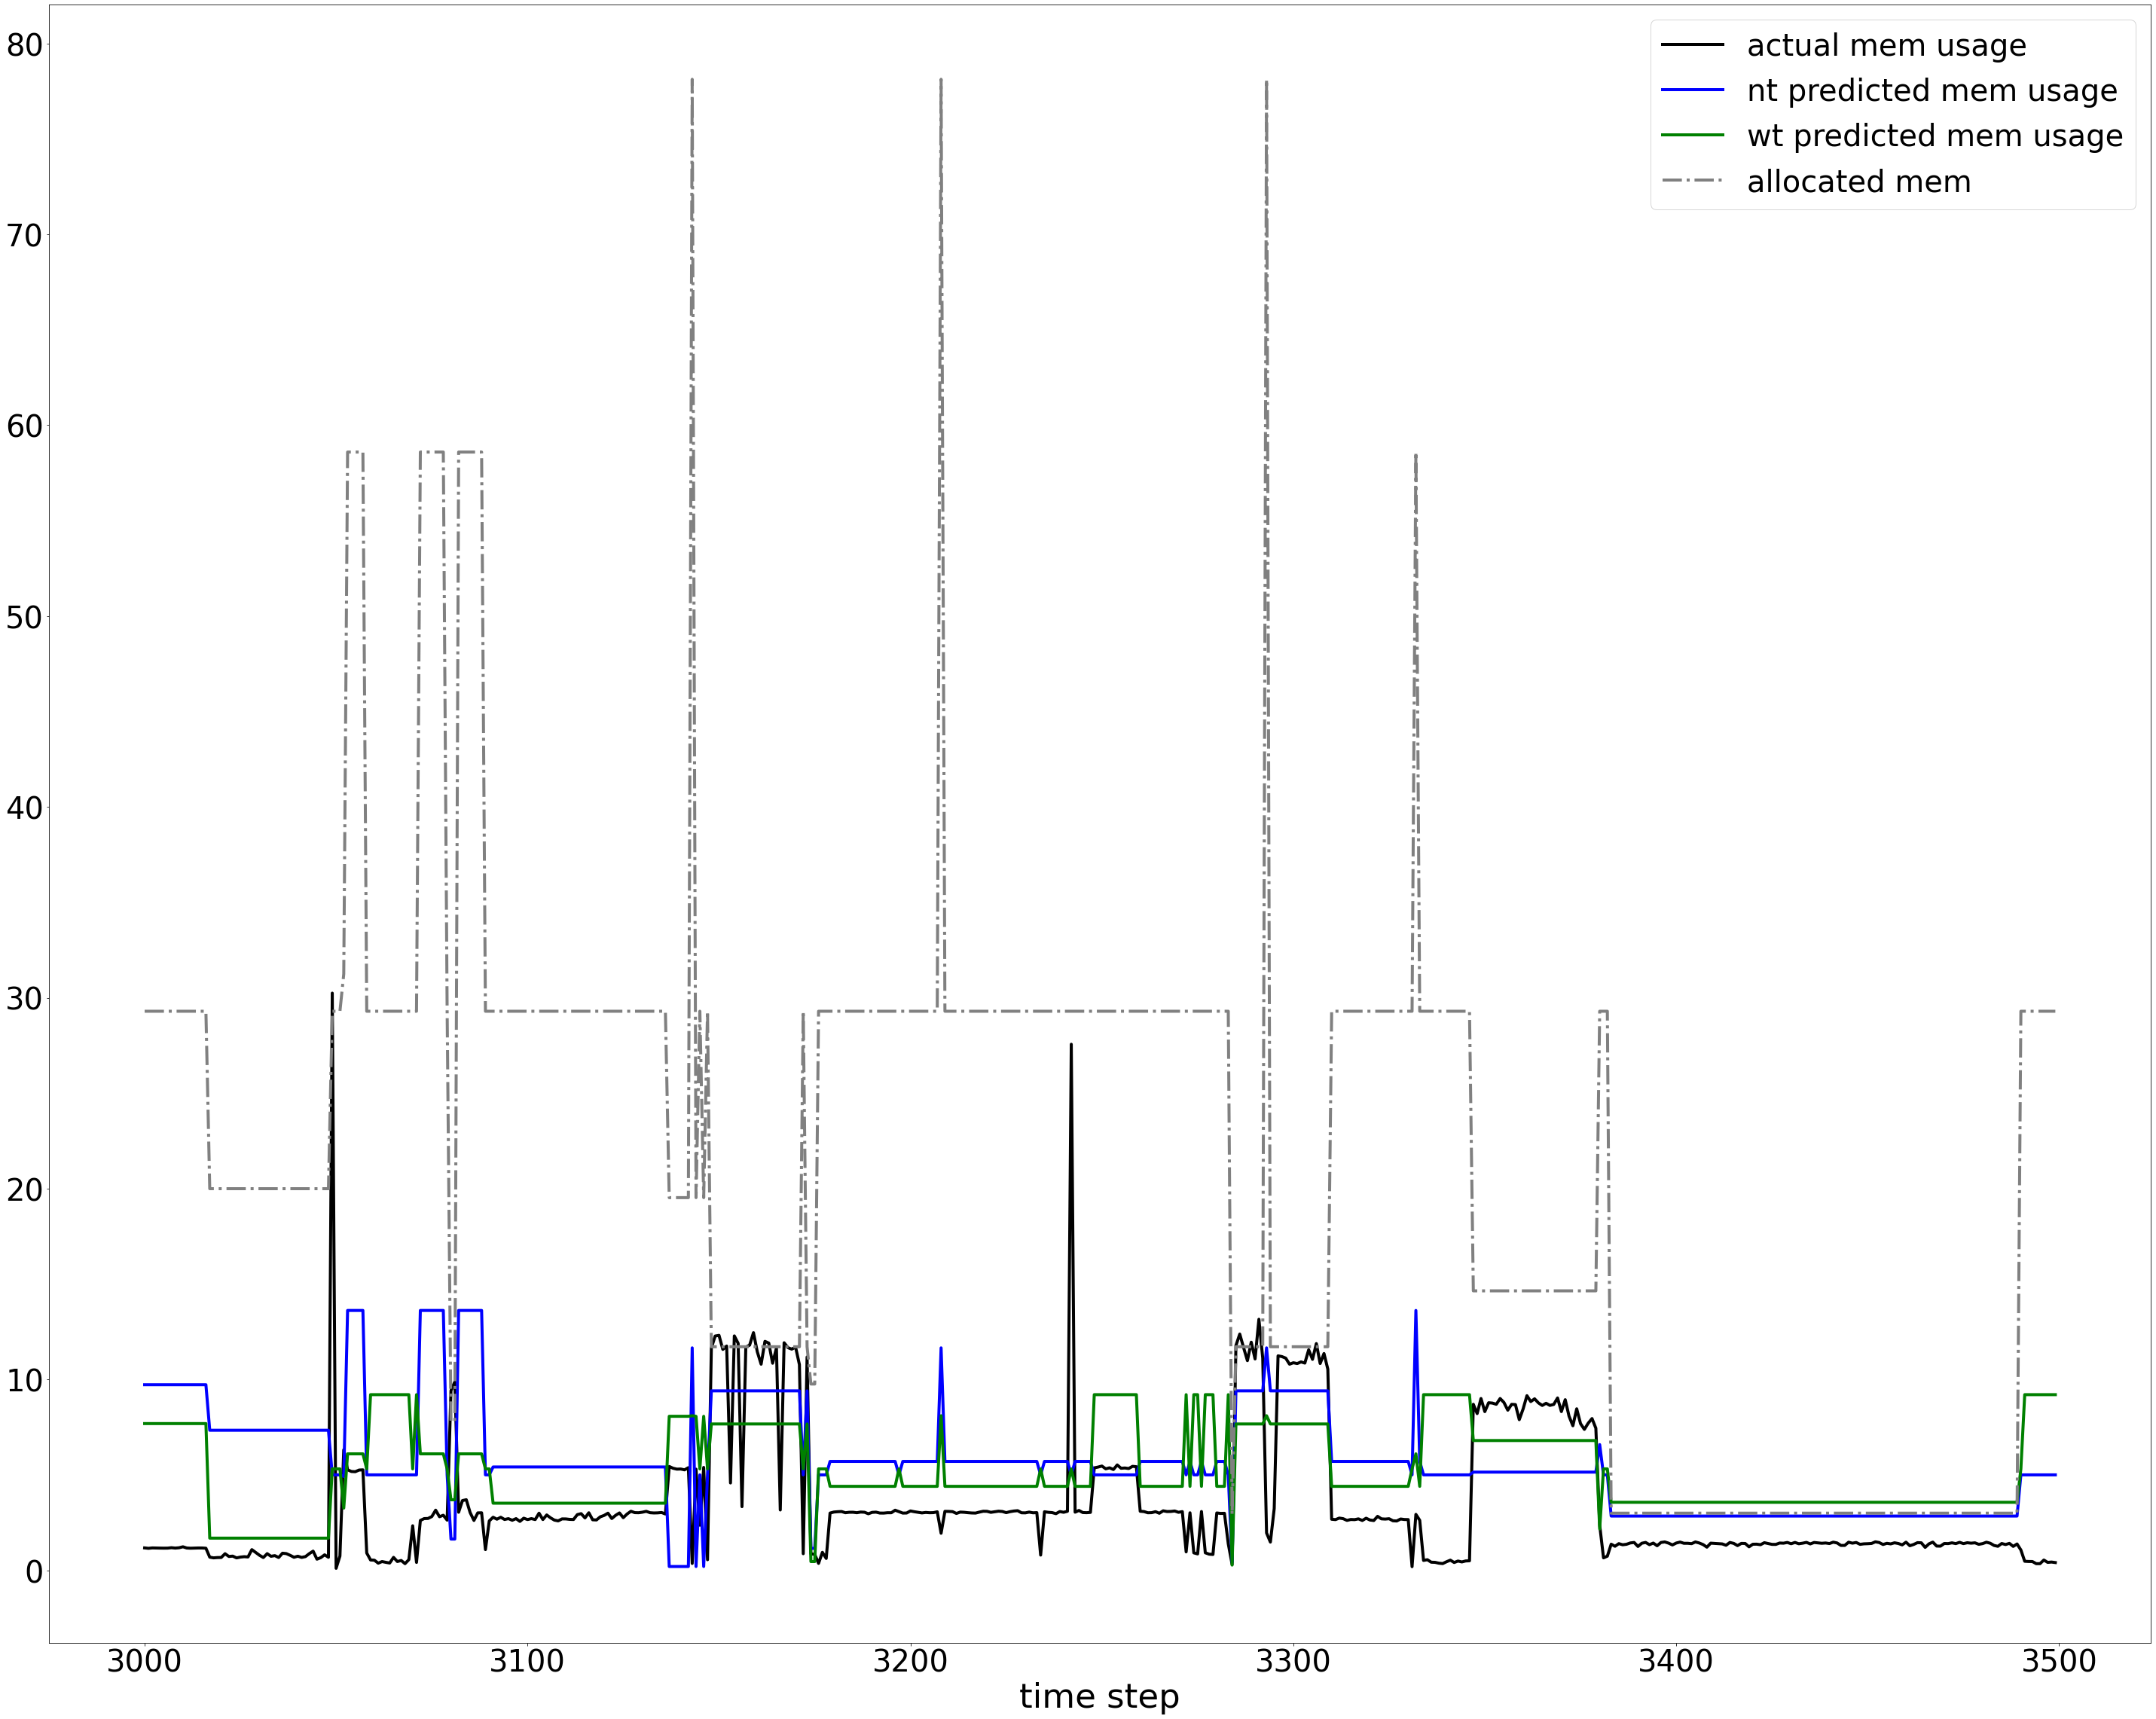
\includegraphics[width=0.85\textwidth]{figures/training_mem_prediction.png}
      \caption{Memory Prediction}
      \label{fig:mem-prediction}
    \end{figure}

  % \section{How much We defer from the Real Value}



  \section{Why We see the Difference}


    Placeholder

    \clearpage



\bibliographystyle{plain} % We choose the "plain" reference style
\bibliography{reference} % Entries are in the refs.bib file



\end{document}

